\subsection{Samarbejde med informanter}

\begin{frame}
\frametitle{Overblik over møder med informanter}
	\begin{itemize}	
		\item Interview 1
		\item Interview 2
		\item Prototype 1A og 1B (lo-fi)
		\item Prototype 2 (hi-fi)
	\end{itemize}
		Møder foregik hos informanterne
\end{frame}

\begin{frame}
\frametitle{Interview 1}
	\begin{itemize}
	\item Om interview 1
			\begin{itemize}
			\item Viden omkring madspild hos informanter
			\item Semistruktureret
			\end{itemize}
	\end{itemize}
\end{frame}

\begin{frame}
\frametitle{Interview 1}
	\begin{itemize}
	\item Resultat af interview 1
			\begin{itemize}
				\item Oplever madspild
				\item Benytter ikke madplan
				\item To systemdefinitioner
			\end{itemize}	
	\end{itemize}
\end{frame}

\begin{frame}
\frametitle{Interview 2}
	\begin{itemize}
	\item Interview 2
			\begin{itemize}
			\item Præsentation af begge systemdefinitioner
			\item Valg af systemdefinition
			\item Krav til systemet $\rightarrow$ tilpasning af systemdefinition
			\end{itemize}
	\end{itemize}
\end{frame}

\begin{frame}
\frametitle{Interview 2}
	\begin{itemize}
	\item Resultat af interview 2
			\begin{itemize}
			\item Systemet bruges på en bærbar
			\item Programmet skal fokusere på hovedretter
			\item Der skal vises billeder af opskrifterne
			\item Opskrifterne skal sorteres efter mængde af passende ingredienser
			\item Opskrifter skal kunne skaleres i forhold til personer
			\item Systemet skal kunne huske ingredienser til næste søgning
			\end{itemize} 
	\end{itemize}
\end{frame}

\begin{frame}
\frametitle{Prototype 1}
	\begin{itemize}
	\item Formål
			\begin{itemize}
			\item Hvordan indsætter en bruger sine råvaretyper?
			\item To løsninger, prototype 1A og 1B
			\item 1A: Indtast navn $\rightarrow$ dropdown med autocompletes
			\item 1B: Vælg kategori $\rightarrow$ underkategori $\rightarrow$ underkategori $\rightarrow$ råvaretype
			\end{itemize} 
	\end{itemize}
\end{frame}


\begin{frame}
	\frametitle{Prototype 1A}
	\begin{figure}
	\centering
	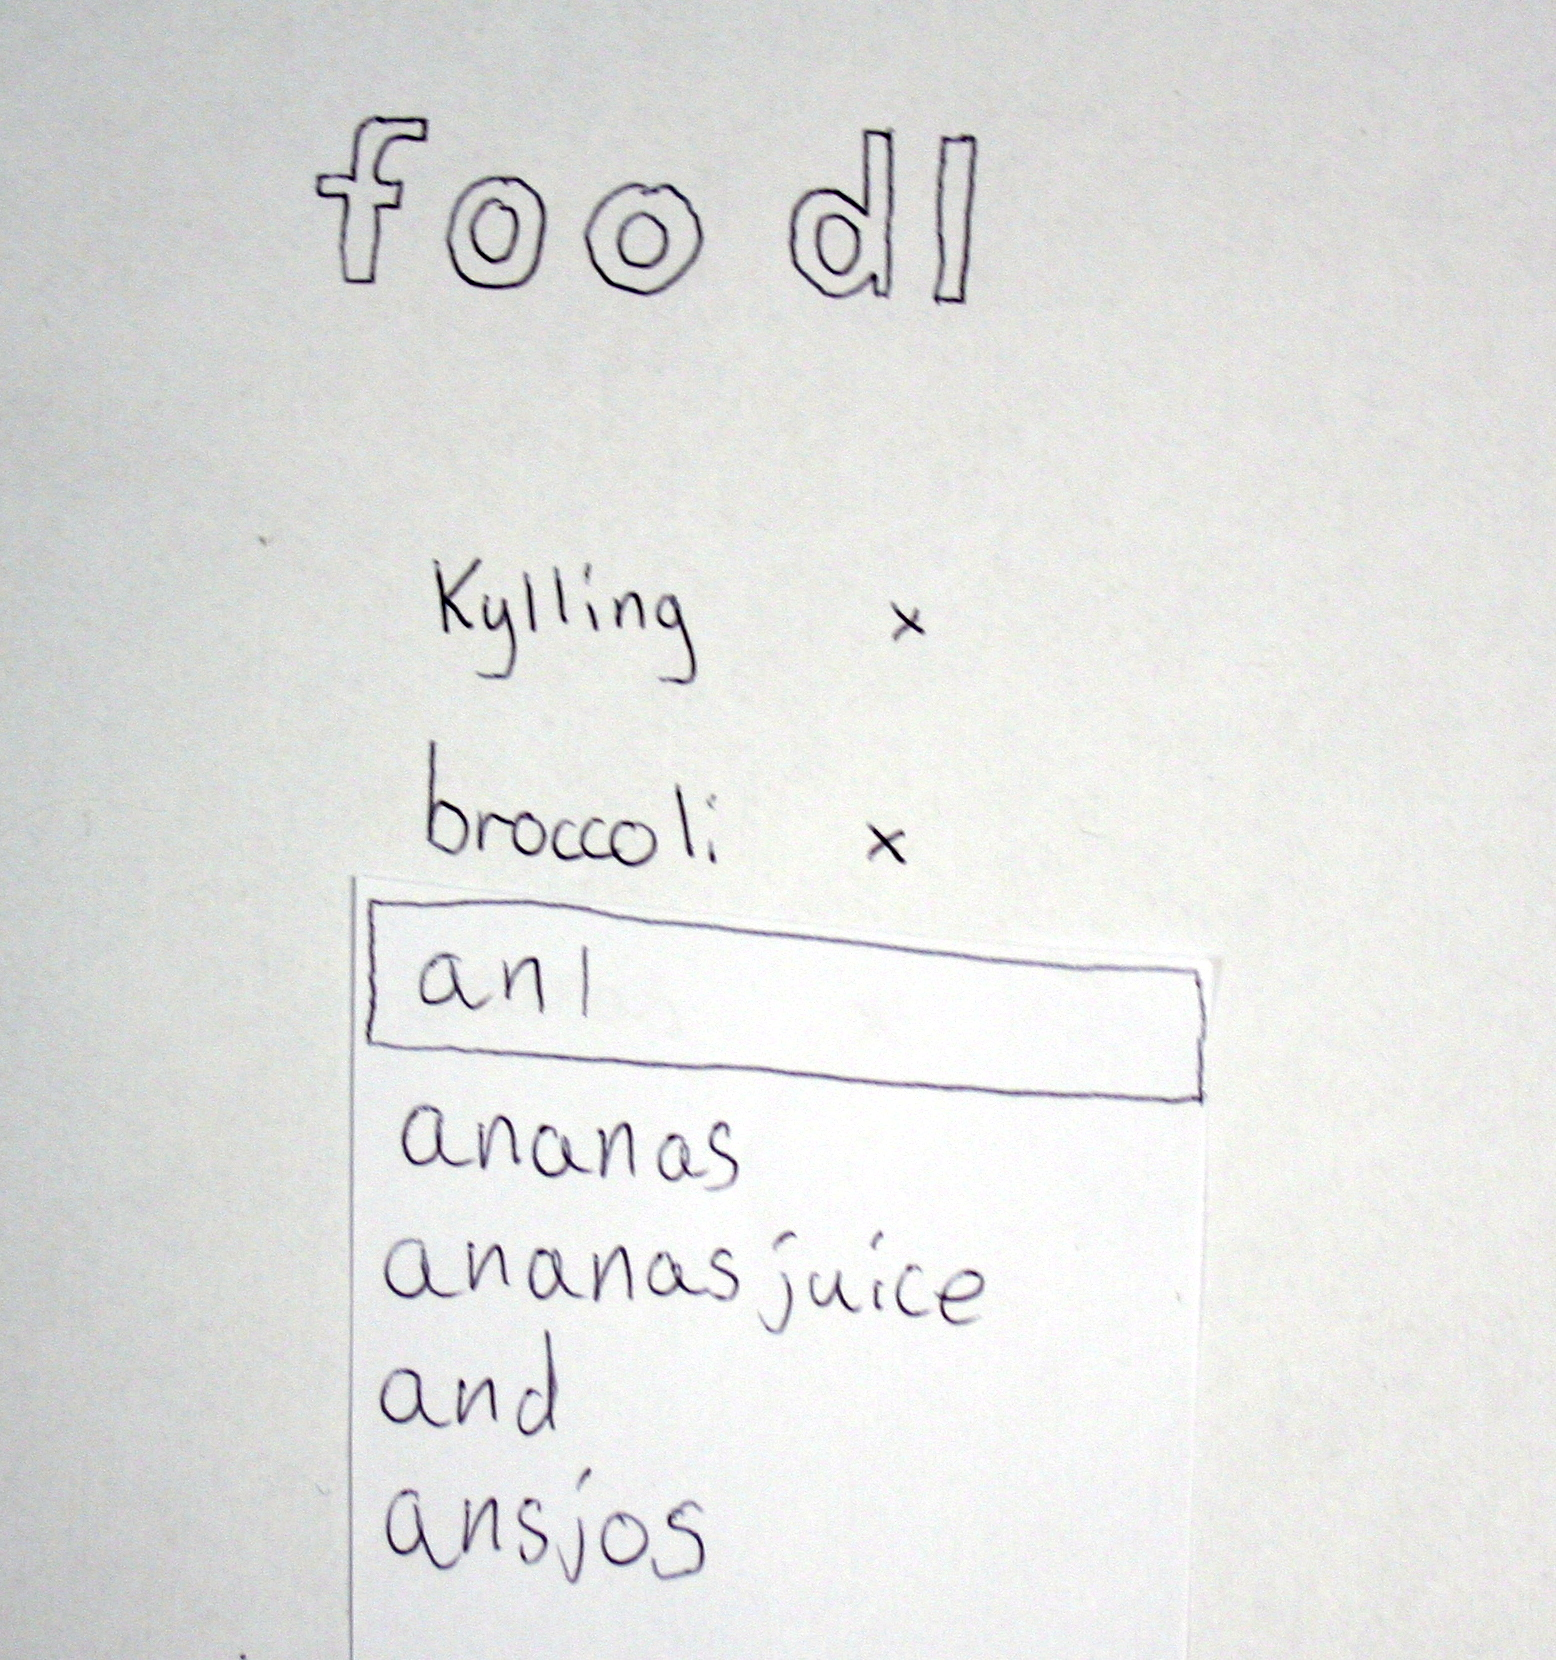
\includegraphics[scale=0.08]{billeder/prototype1a.jpg}
	\caption{Prototype 1A}
	\end{figure}
\end{frame}

\begin{frame}
	\frametitle{Prototype 1B}
	\begin{figure}
	\centering
	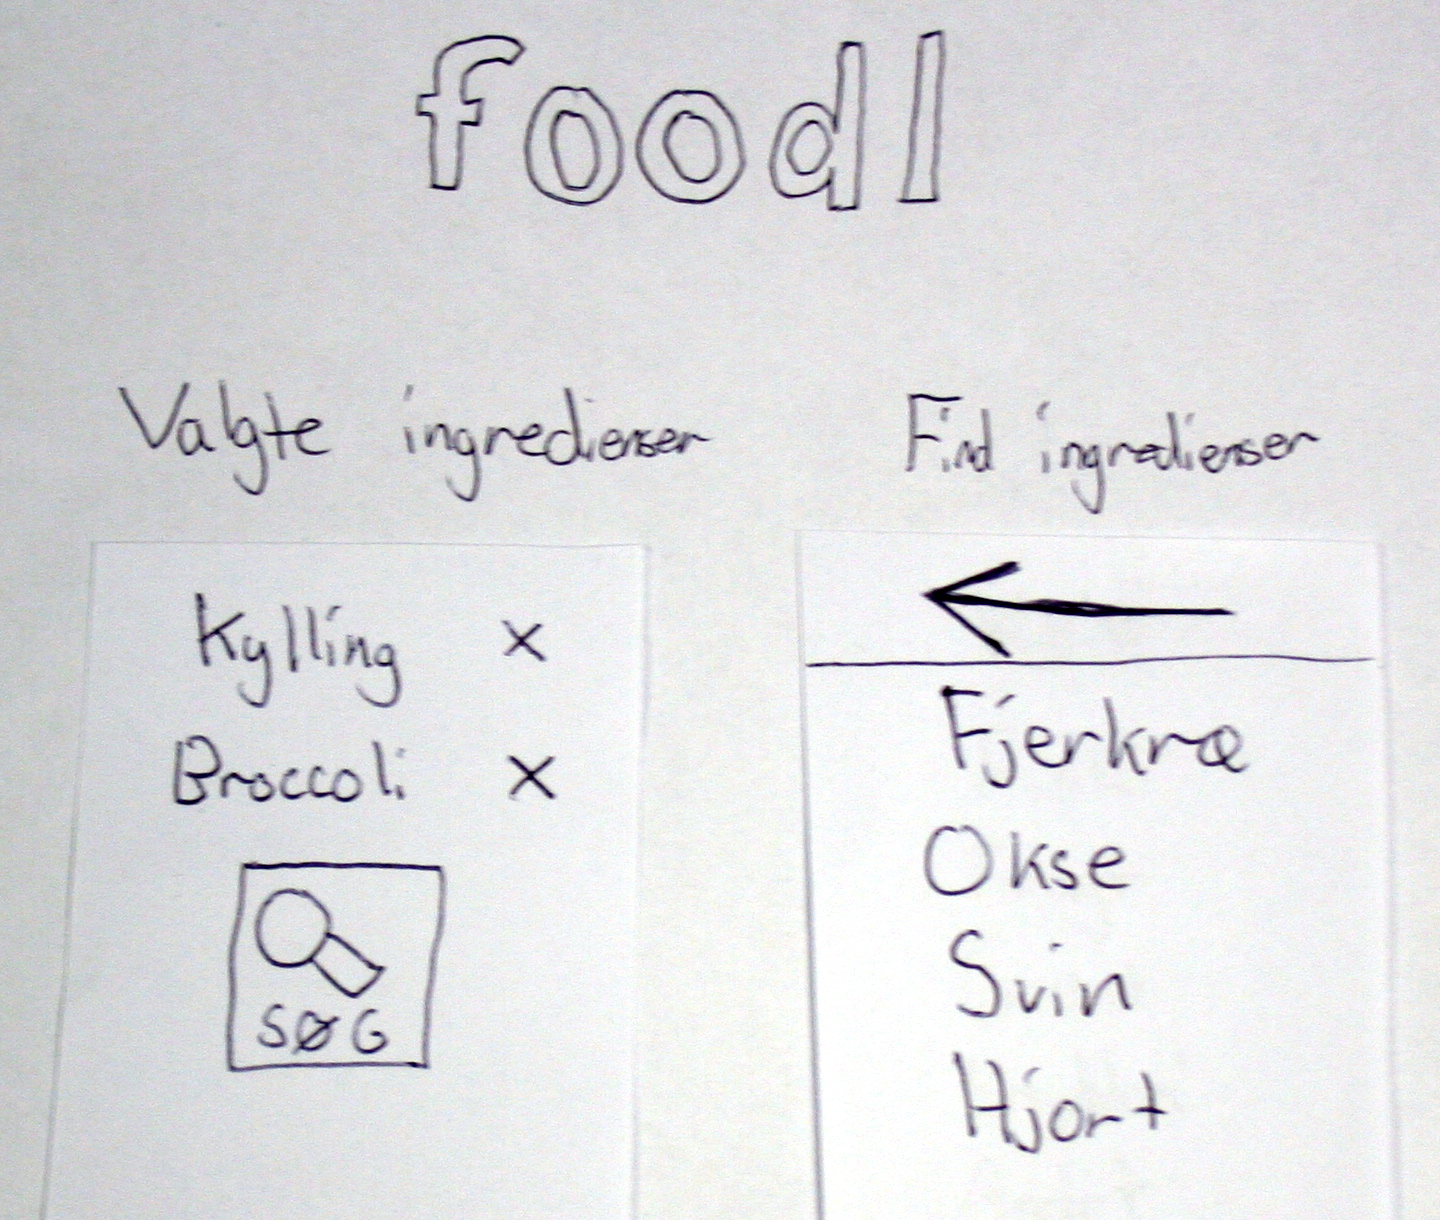
\includegraphics[scale=0.08]{billeder/prototype1b.jpg}
	\caption{Prototype 1B}
	\end{figure}
\end{frame}

\begin{frame}
\frametitle{Bedste prototype}
	\begin{itemize}
	\item Prototype 1A
			\begin{itemize}
			\item Fordele
				\begin{itemize}
				\item Hurtig valg af råvaretyper
				\end{itemize}
			\item Ulemper
				\begin{itemize}
				\item Kræver tastatur
				\end{itemize}
			\end{itemize}
	\item Prototype 1B
			\begin{itemize}
			\item Fordele
				\begin{itemize}
				\item Kræver kun et pegeredskab
				\end{itemize}
			\item Ulemper
				\begin{itemize}
				\item Tvivl om valg af kategori
				\item Lang liste at vælge fra
				\item Langsom valg af råvaretyper
				\end{itemize}
			\end{itemize} 
	\end{itemize}
	
\end{frame}

\begin{frame} %Vinder:
	\frametitle{Bedste prototype}
	\begin{figure}
	\centering
	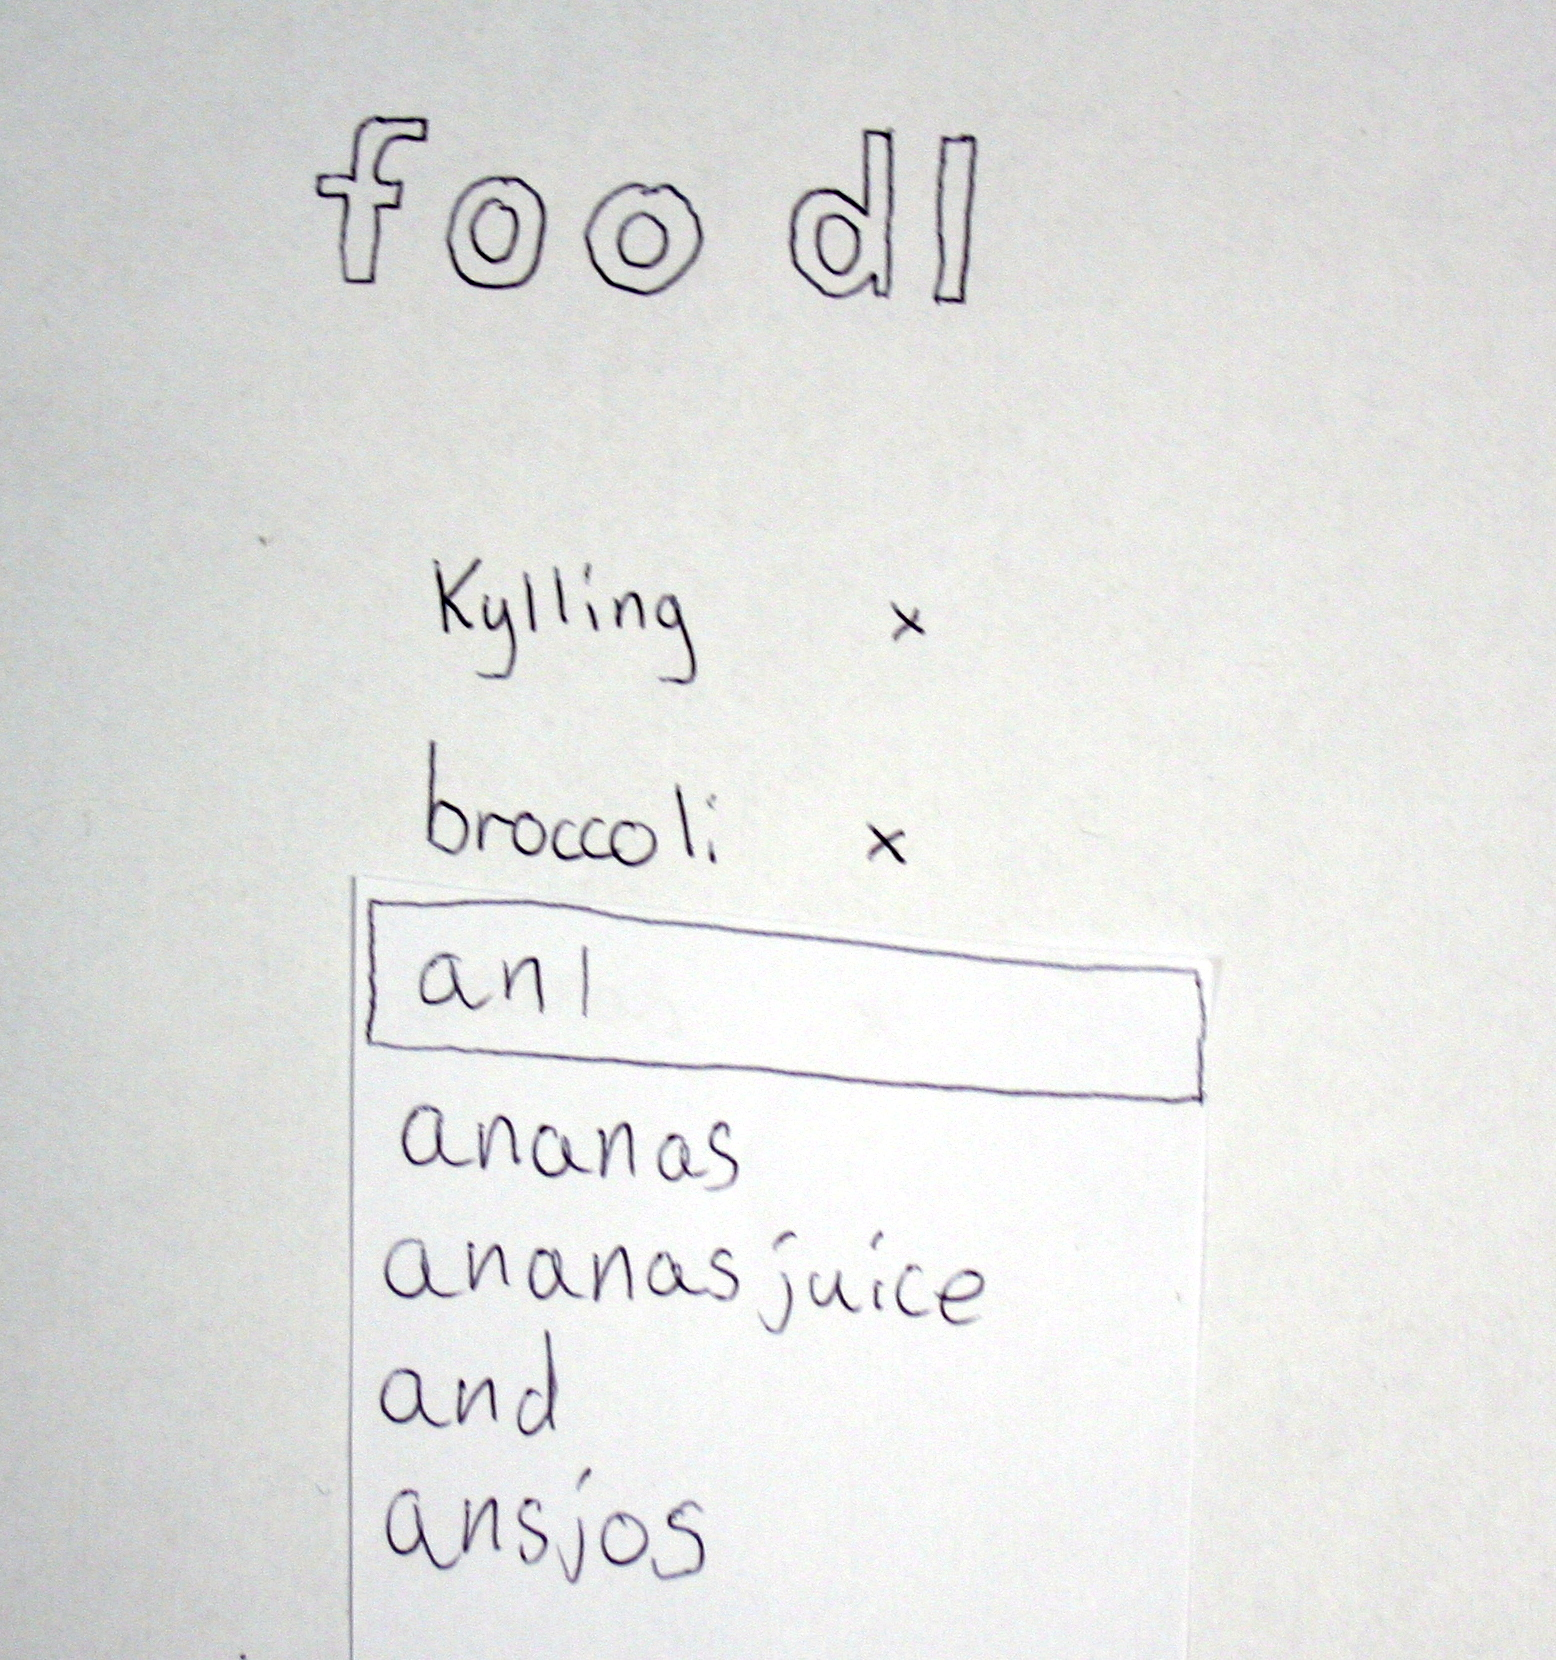
\includegraphics[scale=0.08]{billeder/prototype1a.jpg}
	\caption{Prototype 1A}
	\end{figure}
\end{frame}

\begin{frame}
\frametitle{Prototype 2}
	\begin{itemize}
		\item Hi-fi
		\item Formål
		\begin{itemize}
		\item Krav til funktioner
		\item Sides opbygning
		\end{itemize}
	\end{itemize}
\end{frame}

\begin{frame}
	\frametitle{Prototype 2}
	\begin{figure}
	\centering
	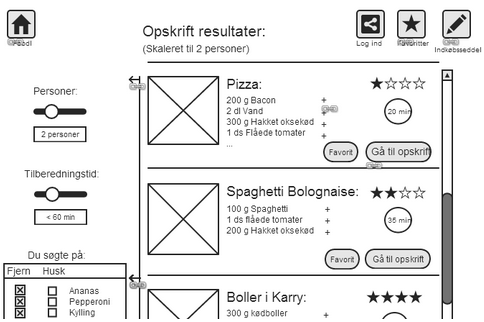
\includegraphics[scale=0.6]{billeder/prototype2.png}
	\caption{Prototype 2}
	\end{figure}
\end{frame}




